% Kapitel zu Daten & Methodik der Hausarbeit

\subsection{Datenbasis}

Wie in der Originalstudie liegt auch hier die der Monitoring of Fund Arrangements (MONA) der IMF zugrunde. Die MONA-Datenbank enthält Informationen zu allen IMF-Programmen, die seit 1990 abgeschlossen wurden. Sie umfasst Angaben zu den Ländern, die an den Programmen teilnehmen, den Zeiträumen der Programme, den finanziellen Bedingungen und den politischen Auflagen, die mit den Programmen verbunden sind. Der Datensatz ermöglicht eine Disaggregierung anhand der Arten von Policy-Konditionen und der Programmtypen, ebenso der Umfang der Konditionalität in Bezug auf Anzahl verschiedener betroffener Policy-Bereiche, die von der KOnditionalität abgedeckt werden. 

Beschreibung der Daten, Zeitraum, Länder, Variablen und Quellen.
% NOTIZ (hier konkretisieren): Stichprobe nennen — 543 Land-Jahre,
% 116 Laender, Panel 1992-2025, Analysezeitraum 1992-2023 (2024/25
% ausgeschlossen; vollstaendige Faelle je Modell abweichend: H1 n=281,
% H2 n=212). Datenquellen zitierfaehig machen: MONA (historisch:
% DSV-Nachbau; ab 2009: Combined_ISO), UNSC-Mitgliedschaft DPPA
% (DPPA-SCMembership.csv), WDI-Kontrollen inkl. Indikator-Codes
% (z. B. DT.DOD.DIMF.CD fuer IMF-Kreditbestand).

Die Quartalsvariable operationalisiert die Programmdauer als die im Sample relevante Anzahl von 90-Tage-Perioden. Dabei wird die Laufzeit durch Rundung auf die nächstliegende ganze Zahl transformiert, damit die Messung mit der Originaldefinition der DSV-Replikation übereinstimmt und kleine Datumsabweichungen nicht als reale inhaltliche Unterschiede interpretiert werden.

„Zeilenzählung ohne Dedup“ bedeutet, dass die ursprüngliche Bedingungszählung auf der Ebene einzelner MONA-Einträge durchgeführt wird, ohne vorab doppelte Einträge zu entfernen. Diese Vorgehensweise ist erforderlich, um die Originalmessung und damit die Validierung gegen den Referezdatensatz exakt zu reproduzieren.

Definition nach Codebook für Rohstoff-Klassifikation:
rohstoff\_final = 1 nur wenn der Gegenstand der Bedingung der Extraktivsektor ist: Öl, Gas, Bergbau, Mineralien, Kraftstoffe — einschließlich fiskalischer Operationen mit explizitem Öl-/Mineral-Bezug (Ölpreis-Fonds, Öl-Parastatal-Zahlungen, Petroleum-Steuer).
Nicht rohstoff: Bank-Privatisierung, allgemeine Export-/Zoll-Bedingungen, Agrar (z. B. „sugar and edible oils“), Strom/Energie ohne Extraktiv-Bezug („energy sector“ → gehört zur breiteren Sensitivitätskategorie, nicht zur engen).

  \subsubsection{Abhängige Variablen}
Bei Dreher et al. Seite 123ff.


  \subsubsection{Unabhängige Variablen}
Bei Dreher et al. Seite 125f.
% SLOT U1 — unsc3-Operationalisierung (2-3 eigene Saetze)
% Behauptung: unsc3 = 1, wenn das Land in Jahr t ODER t+1 temporaeres
% UNSC-Mitglied ist (DSV-Regel, Wahljahr inklusive) — 3-Jahres-Fenster
% aus Wahljahr + 2 Amtsjahren, nicht nur die Amtsjahre.
% Implementierung: code/shared/data_prep/build_unsc_dsv_rule.R
% (DPPA-Vollpanel), im Phase-B-Panel als unsc3 gefuehrt; Dokumentation
% CODEBOOK_MONA.md Abschnitt 10.5. Laenderliste mit Wahljahr/Amtszeit/
% Behandlungsfenster: results/phase_b/tables/phase_b_unsc_mitglieder.csv.
% Abweichung vom Original: Handkorrekturen (AETH 1992, RUS 1995/96/99)
% werden im Vollpanel NICHT angewandt.
% Quelle: \parencite[TODO]{DreherPoliticsIMFConditionality2015} (S. 125f.)


  \subsubsection{Kontrollvariablen}
Bei Dreher et al. Seite 126f. 

% TODO: Umformulieren
Die US-Hilfe wird — abweichend vom Original — auf das BIP zu Marktpreisen bezogen, da die Faktorkosten-Serie des WDI nicht über 2008 hinaus fortgeführt wird; auf den gemeinsamen Jahren (1992–2008) korrelieren beide Varianten mit r = 0,98, die mediane Abweichung beträgt −14 Prozent.

  \subsubsection{Deskriptive Evidenz}
% TODO vor Abgabe: Tabellenform an finale Formatvorlage anpassen (Buchstaben,
% Ausrichtung, ggf. booktabs, Tabellenverzeichnis).
Analog zur Originalstudie (dort Tabelle 1) wird vor den konfirmatorischen Modellen ein deskriptiver Vergleich zwischen temporären UNSC-Mitgliedern und Nicht-Mitgliedern vorangestellt. Die Balkendiagramme bilden wie im Original nur die Gruppenmittelwerte ab; Standardabweichung und Fallzahl stehen unterhalb der Balken, die p-Werte der Welch-t-Tests sind im Paneltitel bzw. unter der Achse vermerkt. In keinem Vergleich ergibt der Welch-t-Test ein signifikantes Ergebnis (alle p $\geq$ 0{,}29). Diese Evidenz ist ausdrücklich deskriptiv: Die p-Werte charakterisieren die Größe der Rohunterschiede, sie testen keine Hypothese und ersetzen die multivariaten Modelle nicht.


\begin{figure}[h]
\centering
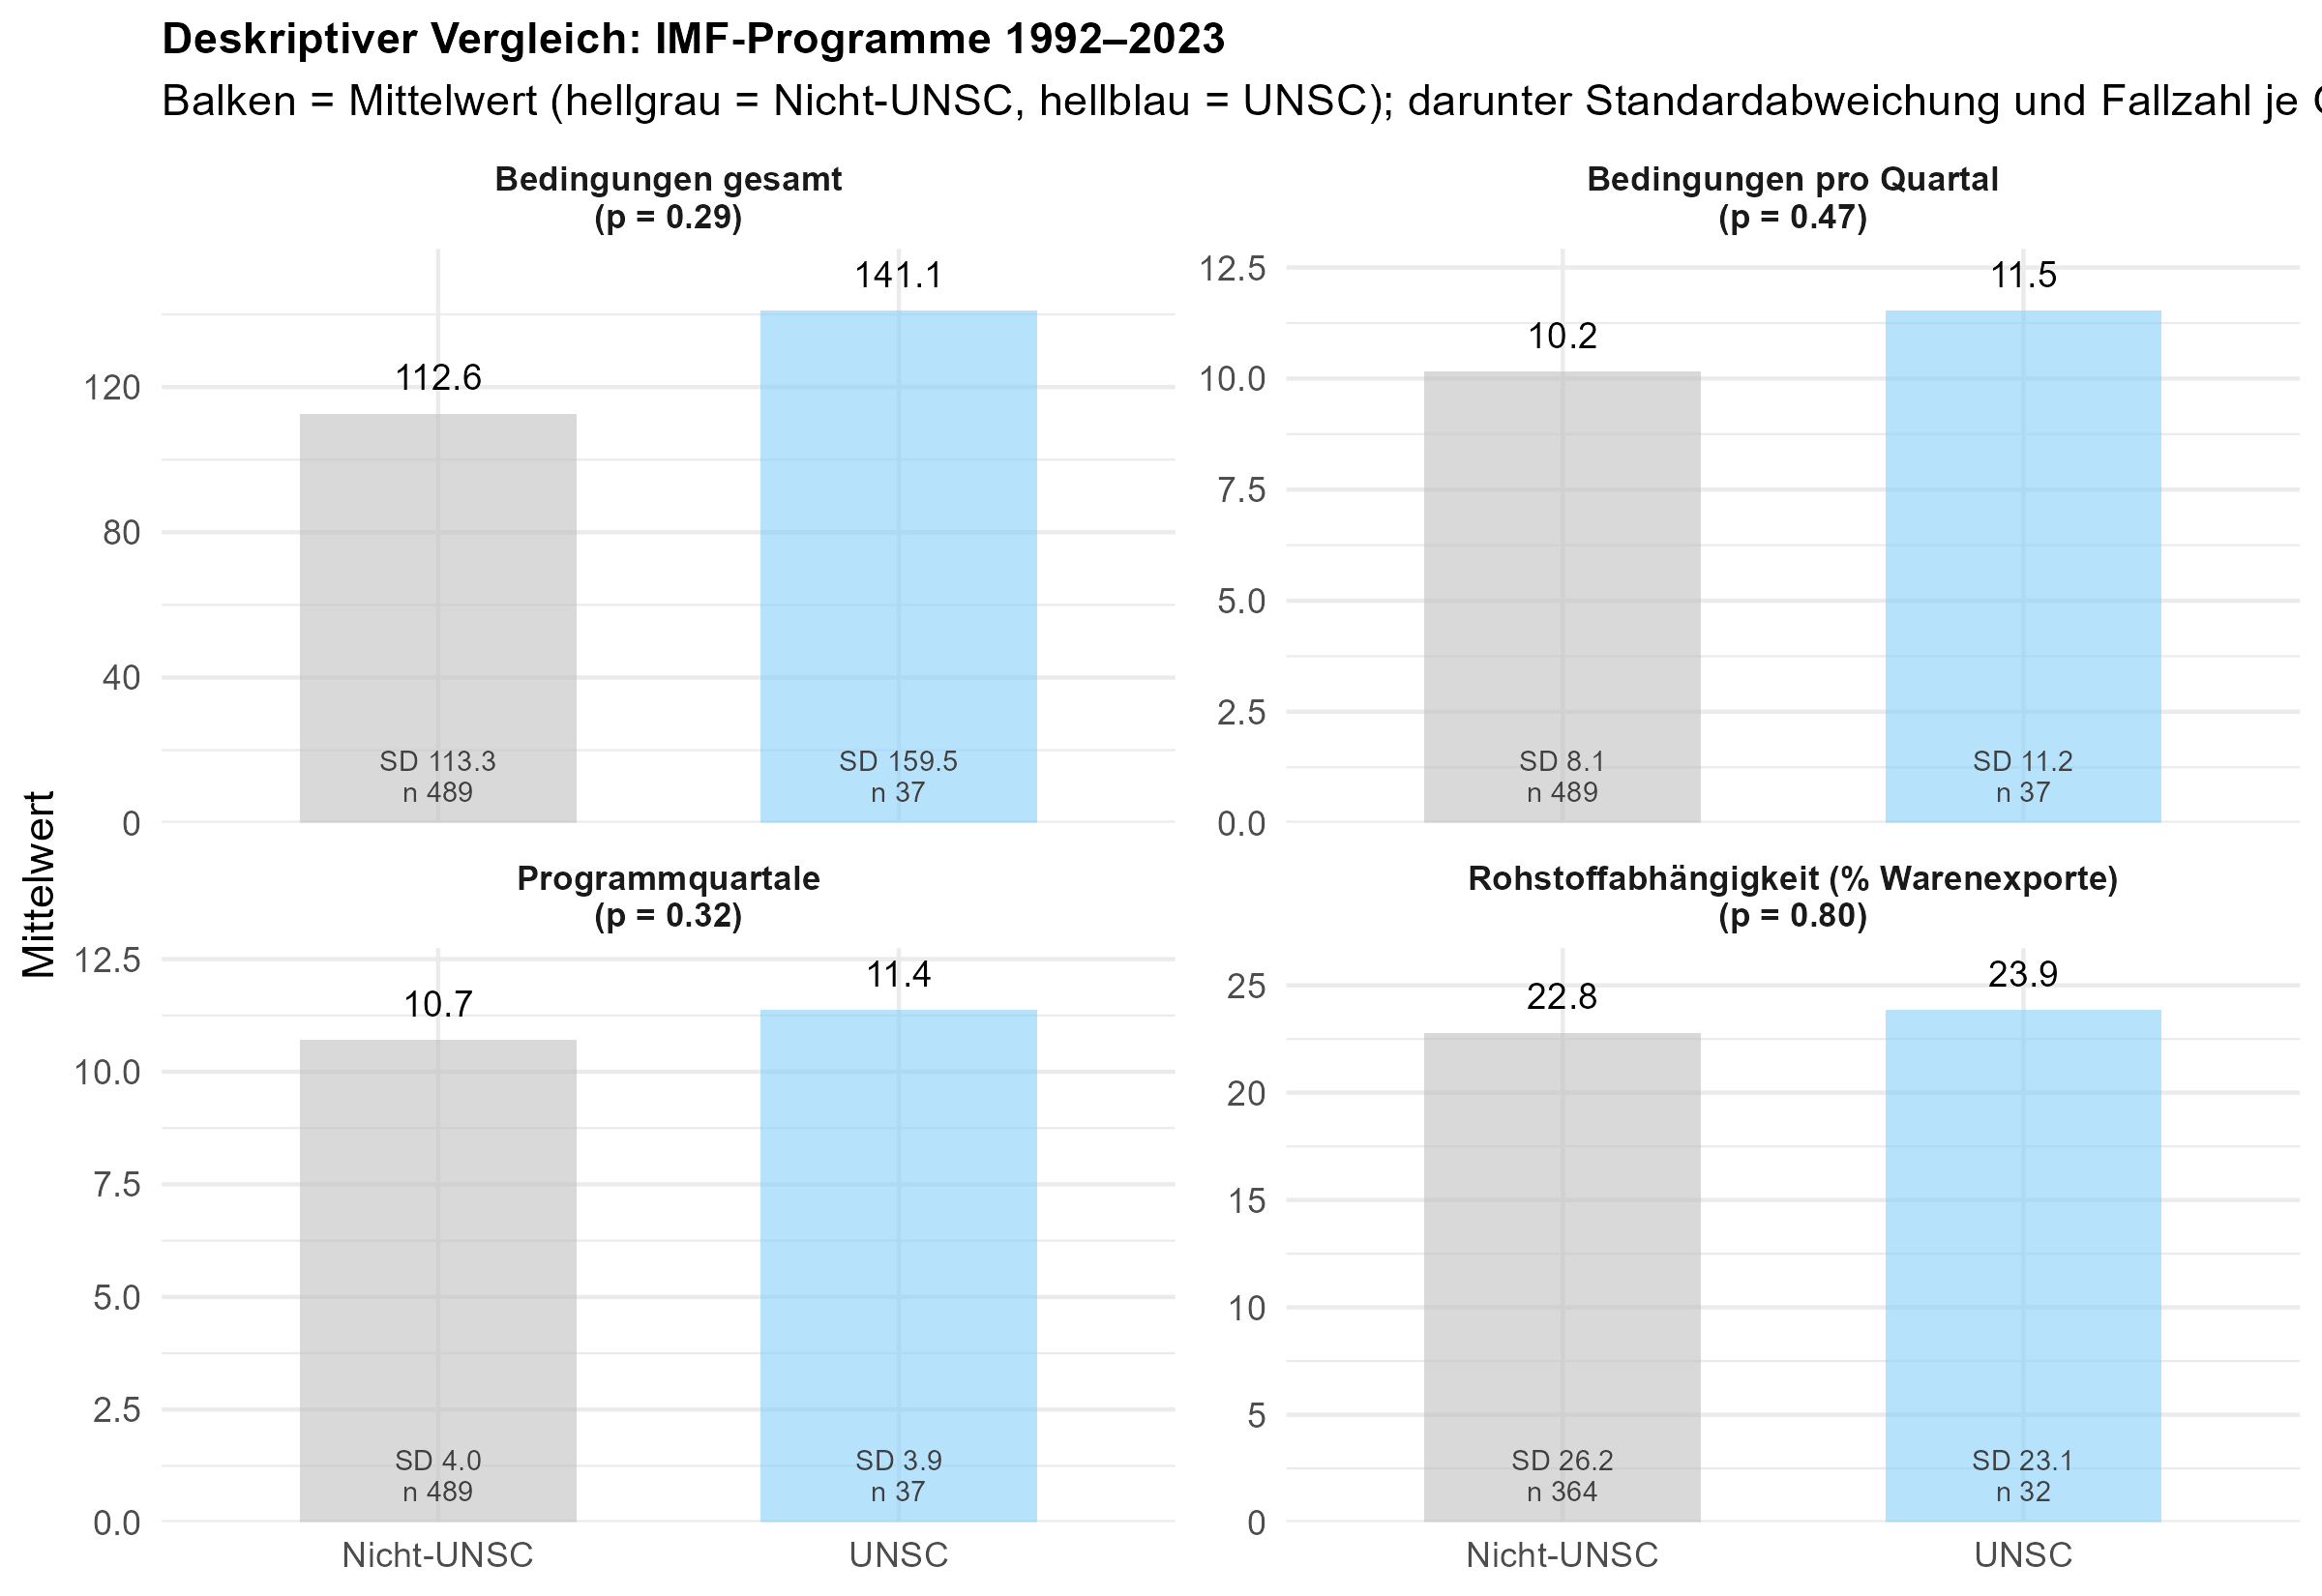
\includegraphics[width=0.85\textwidth]{figures/phase_b/deskriptive_evidenz_gruppe.png}
\caption{Deskriptiver Vergleich UNSC vs.\ Nicht-UNSC, Programm-Land-Jahre 1992--2023 (Balken = Mittelwert; Standardabweichung und Fallzahl je Gruppe unterhalb der Balken; p-Wert des Welch-t-Tests im Paneltitel)}
\end{figure}

Zwei deskriptive Befunde ordnen die Hypothesen ein. Erstens zeigen die \emph{IMF-Programme}, die während einer temporären UNSC-Mitgliedschaft eines Landes bewilligt werden, roh mehr Bedingungen gesamt und eine etwas längere Laufzeit als Programme von Nicht-Mitgliedern; beide Unterschiede sind nicht signifikant. Der Gesamtzähler ist dabei mechanisch laufzeitabhängig: Längere Programme durchlaufen mehr Review-Runden und nehmen mehr Bedingungen auf. Über die Intensität der Konditionalität sagt er deshalb wenig aus; maßgeblich sind die Bedingungen pro Quartal und die Kontrolle der Programmdauer im Modell. Der negativen Erwartung von H1 steht die Rohverteilung damit nicht direkt entgegen, sondern verweist darauf, dass der erwartete Effekt ein Nettoeffekt unter Kontrolle von Programmdauer und Wirtschaftsstruktur ist; wie im Original entsteht der geschätzte Zusammenhang erst in den multivariaten Modellen. Zweitens unterscheiden sich UNSC- und Nicht-UNSC-Jahre in der Rohstoffabhängigkeit praktisch nicht (p um 0{,}8): Die Interaktionsprüfung in H2 wird durch Niveauunterschiede der Rohstoffstruktur nicht vorstrukturiert.

Für H2 wird derselbe deskriptive Vergleich zusätzlich getrennt nach niedriger und hoher Rohstoffexportabhängigkeit (Median-Split, Median 11{,}8 Prozent der Warenexporte) berichtet:

\begin{figure}[h]
\centering
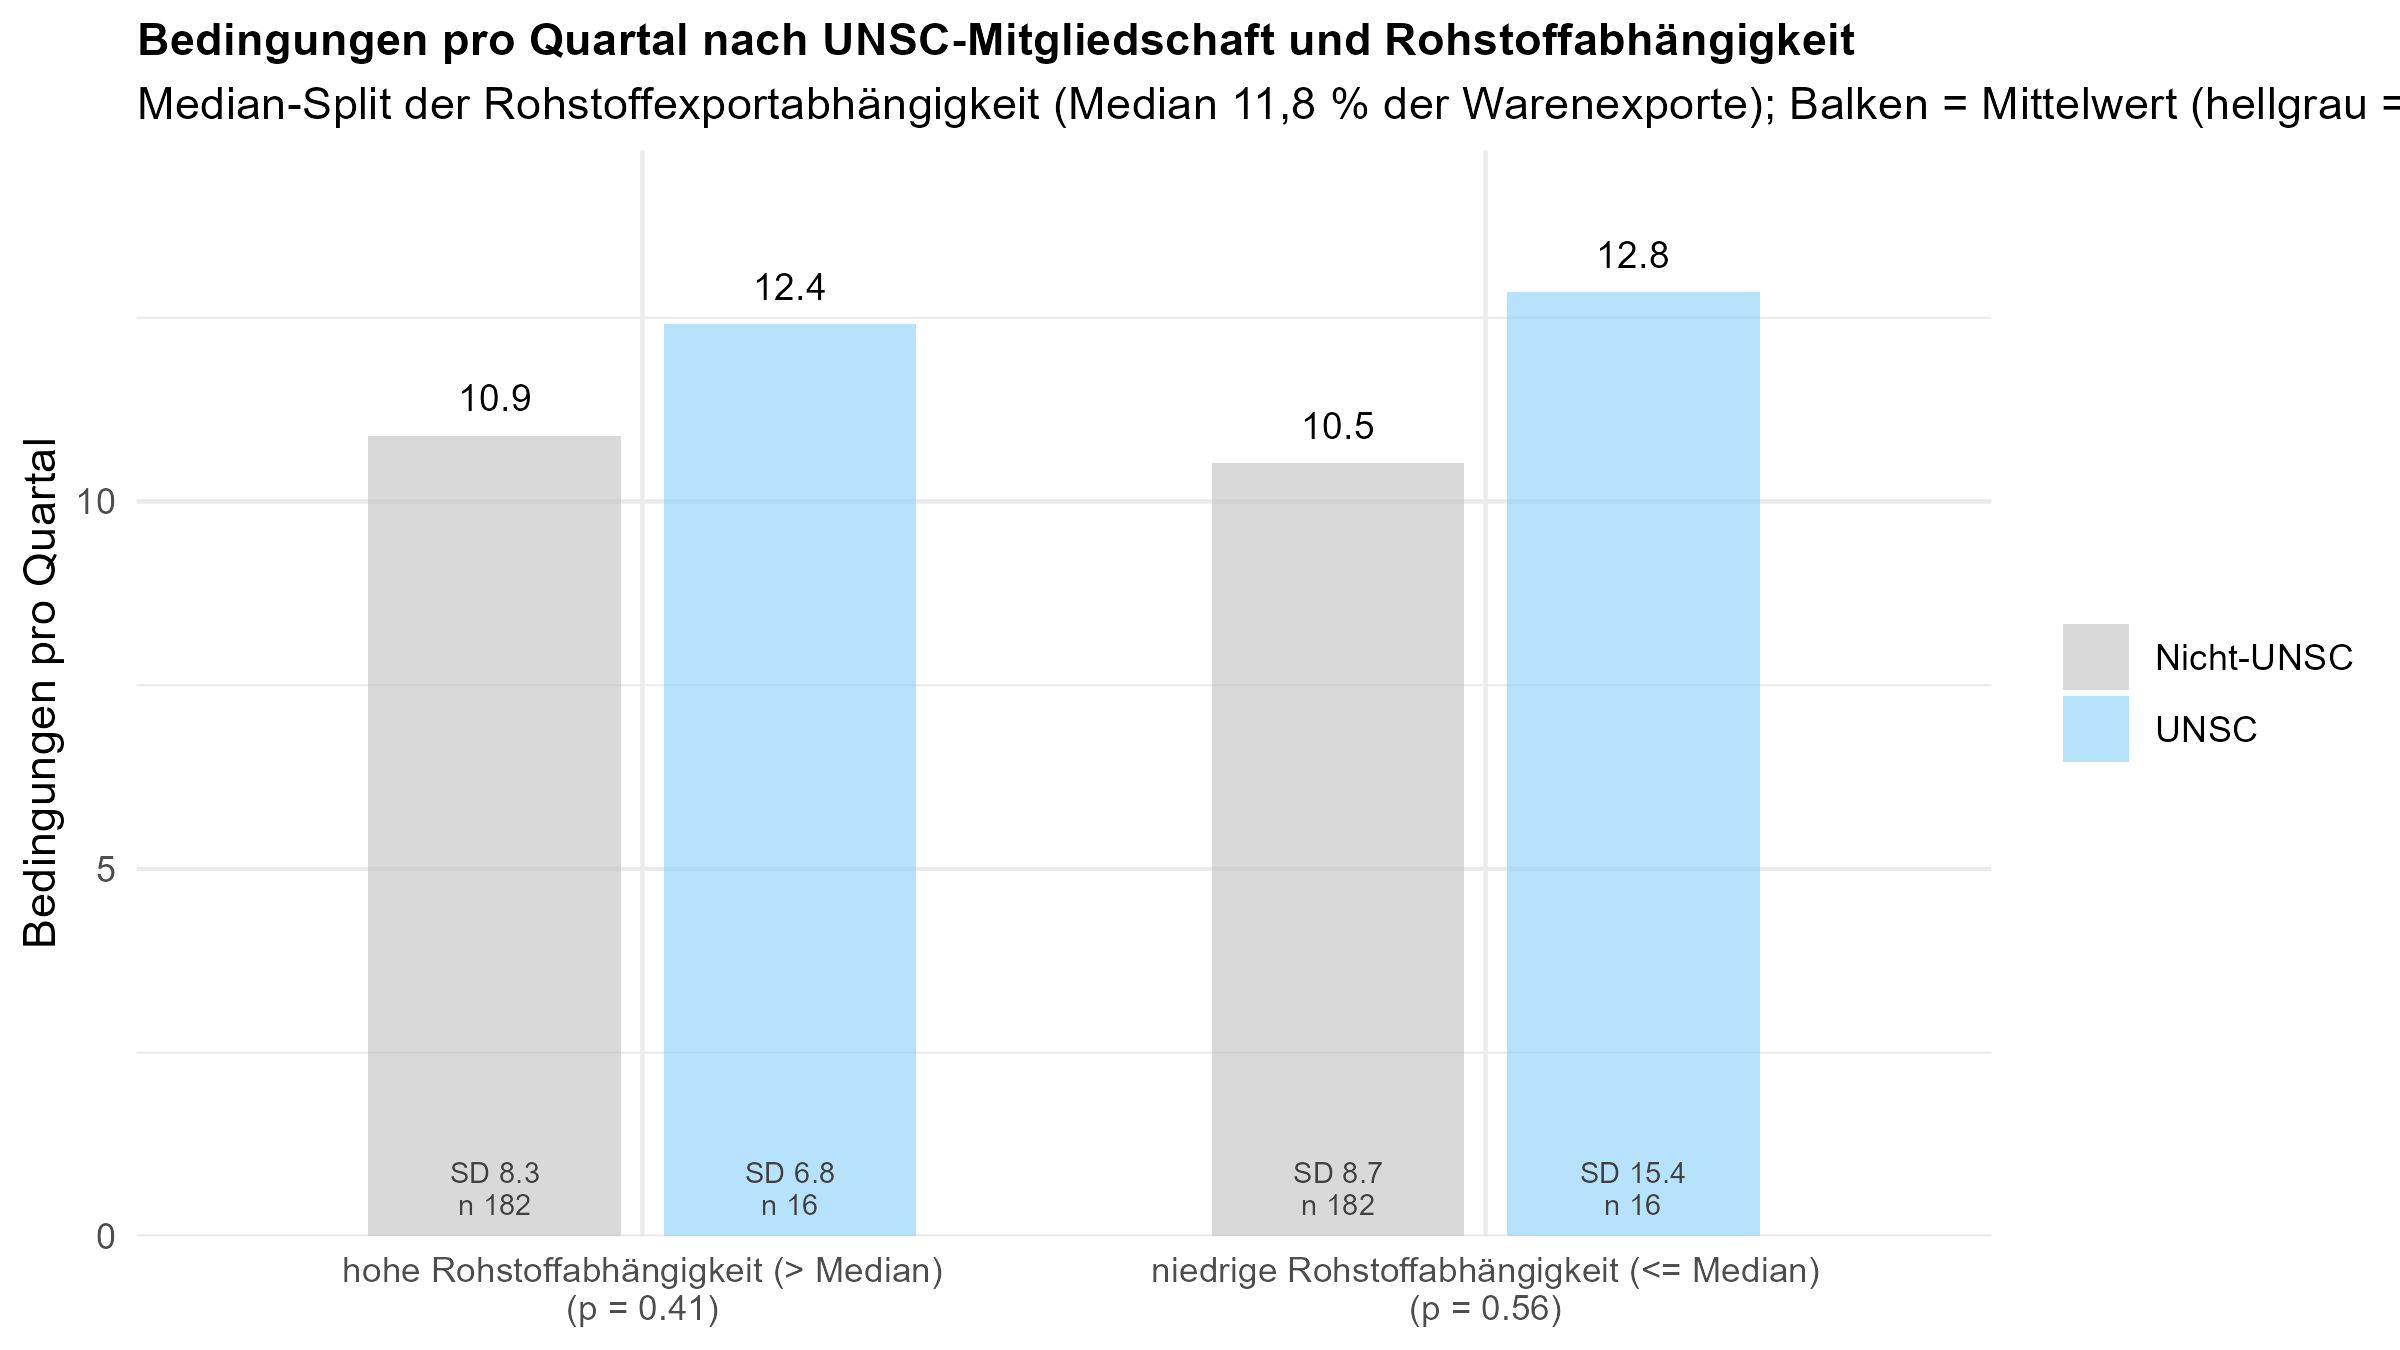
\includegraphics[width=0.85\textwidth]{figures/phase_b/deskriptive_evidenz_h2_split.png}
\caption{Bedingungen pro Quartal nach UNSC-Mitgliedschaft, getrennt nach Rohstoffabh\"angigkeit (Median-Split, Median 11{,}8 Prozent der Warenexporte; Balken = Mittelwert; Standardabweichung und Fallzahl unterhalb der Balken; p-Werte der Welch-t-Tests unter der Achse)}
\end{figure}

Auch hier zeigen sich keine signifikanten Rohunterschiede; die UNSC-Zellen sind klein (je 16 Land-Jahre), sodass die Aufteilung allein der Beschreibung dient.
% Repo-Quelle der Kennzahlen (N je Variable: 489/37 fuer Zaelle und Quartale,
% 364/32 fuer resource_dep, Complete Cases Median-Split: 182/16 je Gruppe):
% code/phase_b/analysis/phase_b_deskriptive_evidenz.R
% results/phase_b/tables/phase_b_deskriptive_evidenz.csv
% results/phase_b/tables/phase_b_deskriptive_evidenz_h2_split.csv



\subsection{Messung und Modellstrategie}
Hier die Operationalisierung, abhängige und unabhängige Variablen sowie Schätzmodell(e) beschreiben.

% TODO vor Abgabe: Formulierung
Die saubere Reihenfolge in der Hausarbeit: H1 und H2 konfirmatorisch testen und als Ihre Ergebnisse berichten → die Quartils-Tabelle im Anhang oder in der Beschreibung der Daten als Kontext („die Programme rohstoffreicher Länder unterscheiden sich inhaltlich“) → und wenn Sie möchten, im Ausblick formulieren: „Für eine künftige Studie böte sich an, die Kompositionshypothese konfirmatorisch zu prüfen, sobald eine belastbarere Klassifikation vorliegt.“ Genau deshalb steht die Bemerkung auch schon so in daten-methodik.tex.

% TODO vor Abgabe: Diese Anmerkung final formulieren oder als
% Robustheits-/Einordnungsabsatz in die Ergebnisse/Diskussion übernehmen.
\paragraph{Anmerkung: Arrangement-Typen und Policy-Areas im Hypothesendesign}
Arrangement-Typen (EFF, PRGF, SBA) und die Verteilung der Bedingungen auf Policy-Areas stehen zwar inhaltlich im Zusammenhang mit Rohstoffabhängigkeit und Stabilisierungsanforderungen. Sie wurden jedoch bewusst nicht als Regressoren oder abhängige Variablen in die konfirmatorischen Hypothesentests (H1, H2) aufgenommen. Dafür gibt es drei Gründe:
\begin{enumerate}
  \item Die klassifikationsbasierte Analyse rohstoff- bzw. stabilitätsbezogener Auflagen entspricht der früheren vierten Hypothese. Sie wurde wegen der unsicheren Operationalisierung aus dem konfirmatorischen Pfad genommen: Die Klassifikation beruht auf einer deterministischen Textregel, und 417 historische MONA-Zeilen ohne Beschreibungstext werden nach der Regel \glqq kein Textsignal = 0\grqq{} als nicht rohstoffbezogen kodiert. Eine Messregel mit dieser Fehleranfälligkeit trägt keinen konfirmatorischen Test und wird ausschließlich explorativ berichtet.
  \item Arrangement-Typen sind potenzielle Mediatoren (post-treatment): Die Fazilität wird zwischen IWF und Land verhandelt. Würde die UNSC-Mitgliedschaft oder die Rohstoffabhängigkeit beeinflussen, welche Fazilität ein Land erhält, würde eine Kontrolle für den Typ den zu schätzenden Gesamteffekt teilweise wegkontrollieren. Auch die Originalstudie nutzt die Arrangement-Typen deshalb nur deskriptiv und zur Stichprobenaufteilung, nicht als Kontrollen im Hauptmodell.
  \item Kompositionsanalysen (welche Policy-Areas von den Bedingungen betroffen sind) wären eigene abhängige Variablen. Für den modernen Zeitraum ab 2009 fehlt eine DSV-identische Messung, weil die Zuordnung moderner MONA-Bedingungen zu den 20 Policy-Areas dieselbe Klassifikationsunsicherheit wie die Rohstoffregel aufweist.
\end{enumerate}
H1 und H2 testen deshalb den Gesamtumfang der Konditionalität (Bedingungen pro Quartal). Die Komposition der Bedingungen wird rein deskriptiv ausgewertet: als Anteil der als rohstoff- bzw. stabilitätsrelevant klassifizierten Bedingungen nach Quartilen der Rohstoffexportabhängigkeit. Ein nachträgliches konfirmatorisches Deuten solcher Kompositionsanalysen würde zudem gegen das Prinzip vorab spezifizierter Hypothesen verstoßen (HARKing); sie sind wie die H3-Länderprofile klar als explorativ zu kennzeichnen.
% Repo-Quelle der deskriptiven Kennzahlen:
% code/phase_b/analysis/phase_b_komposition_exploration.R
% results/phase_b/exploration/komposition_ressourcen_quartile.csv
% results/phase_b/exploration/komposition_ressourcen_quartile_unsc3.csv

\subsection{Abweichungen vom Original und Limitationen}
% ----------------------------------------------------------------------
% SLOT M1 — Abweichungen vom Original (1 Absatz eigene Saetze)
% Muss-Aufzaehlung, alle Punkte im Repo dokumentiert:
% 1. Zeitraum: Phase B 1992-2023 (Panel bis 2025), Original 1992-2008.
% 2. US-Hilfe auf BIP zu Marktpreisen statt Faktorkosten (WDI-Serie endet
%    2008); gemeinsame Jahre 1992-2008: r = 0,98, mediane Abweichung
%    -14 Prozent (steht als TODO bei den Kontrollvariablen).
% 3. Zaehlbasis: ZAehlung ohne Dedup (steht schon in der Datenbasis).
% 4. Handkorrekturen des Originals nicht angewandt (s. SLOT U1).
% 5. H3/H4 nur explorativ: deterministische Textregel; 417 historische
%    MONA-Zeilen ohne Beschreibungstext werden als nicht rohstoffbezogen
%    kodiert (s. Anmerkung-Absatz zu Arrangement-Typen unten).
% 6. AV: Bedingungen pro Quartal statt Gesamtzaehler — der Gesamtzaehler
%    ist laufzeitmechanisch (s. deskriptive Evidenz).
% 7. Zwei-Wege-FE (Laender- UND Jahres-FE) als Hauptspezifikation ist
%    eine bewusste ERGAENZUNG gegenueber DSV (Original-Tabelle 2 ohne
%    Jahres-FE): beggruenden (Epochen-/Krisenjahre absorbieren) und die
%    DSV-nahe GLS-Alternative im Modellvergleich (Anhang) nennen.
% 8. Poisson-FE-Robustheit (H1) folgt Tabelle S2 des Originals
%    (Semi-Elastizitaet, Offset log Quartale).

% SLOT M2 — Limitationen fuer die Auswertung (1 Absatz eigene Saetze)
% Behauptung: kleine UNSC-Zellen beschraenken die statistische Power
% (H2-Vollmodell: 21 unsc3-Jahre in 16 Laendern; Median-Split je 16
% Land-Jahre); Klassifikationsunsicherheit der Rohstoffregel, insbesondere
% post-2008; MONA-Beschreibungstexte historisch uneinheitlich. Deshalb
% Interpretation der Interaktionsmodelle nur vorsichtig-deskriptiv,
% keine kausale Lesart.

\subsection{Robustheitschecks}
Angaben zu Alternative Spezifikationen, Sensitivitätsanalysen oder Heterogenitätschecks.
% NOTIZ (Robustheitsbattery auflisten, s. README-Ergebnistabelle):
% H2: Fuel-/Mineral-Exportvarianten, Placebo Gesamtexporte,
% Winsorisierung (1./99. Perzentil), IMF-Kreditbestand statt
% Nettofluesse; H1: IMF-Kreditbestand, Poisson-FE (S2-Analog),
% Original-Handkorrekturen unsc3 nachgezogen (H1 identisch, H2 in
% 5. Dezimalstelle unveraendert — Kodierungsabweichung ohne Einfluss);
% H2-Zeitfenster 1992-2008 / 2009-2023 (Richtung dreht: +0,274 p=0,012
% bzw. -0,377 p=0,072 — Haupttest bleibt der Gesamtzeitraum);
% Leave-one-country-out (Anhangstabelle).
	
